\begin{figure}[H]
\begin{changemargin}{0cm}{0cm}
  \begin{center}
    \begin{minipage}[h]{0.45\linewidth}
        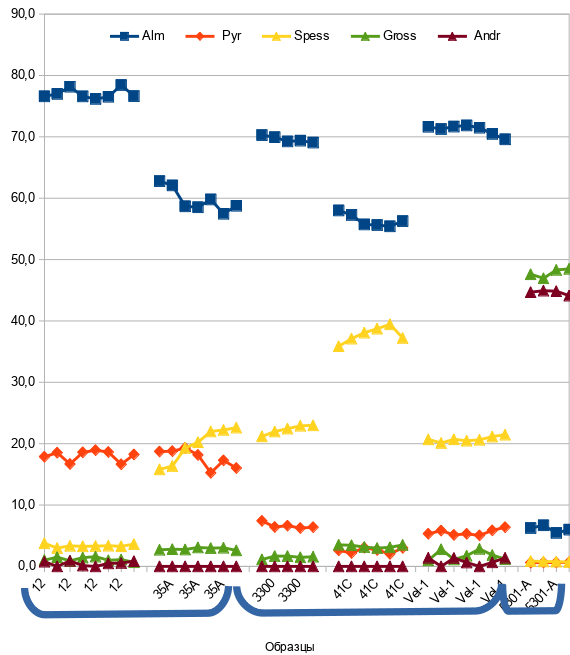
\includegraphics[width=1\textwidth]{authors/polzunenkov-fig2.png}
        \caption{Миналы изученных зёрен гранатов}
        \label{fig:polzunenkov-fig2}
    \end{minipage}
\hfill
    \begin{minipage}[h]{0.5\linewidth}
      \begin{center}
              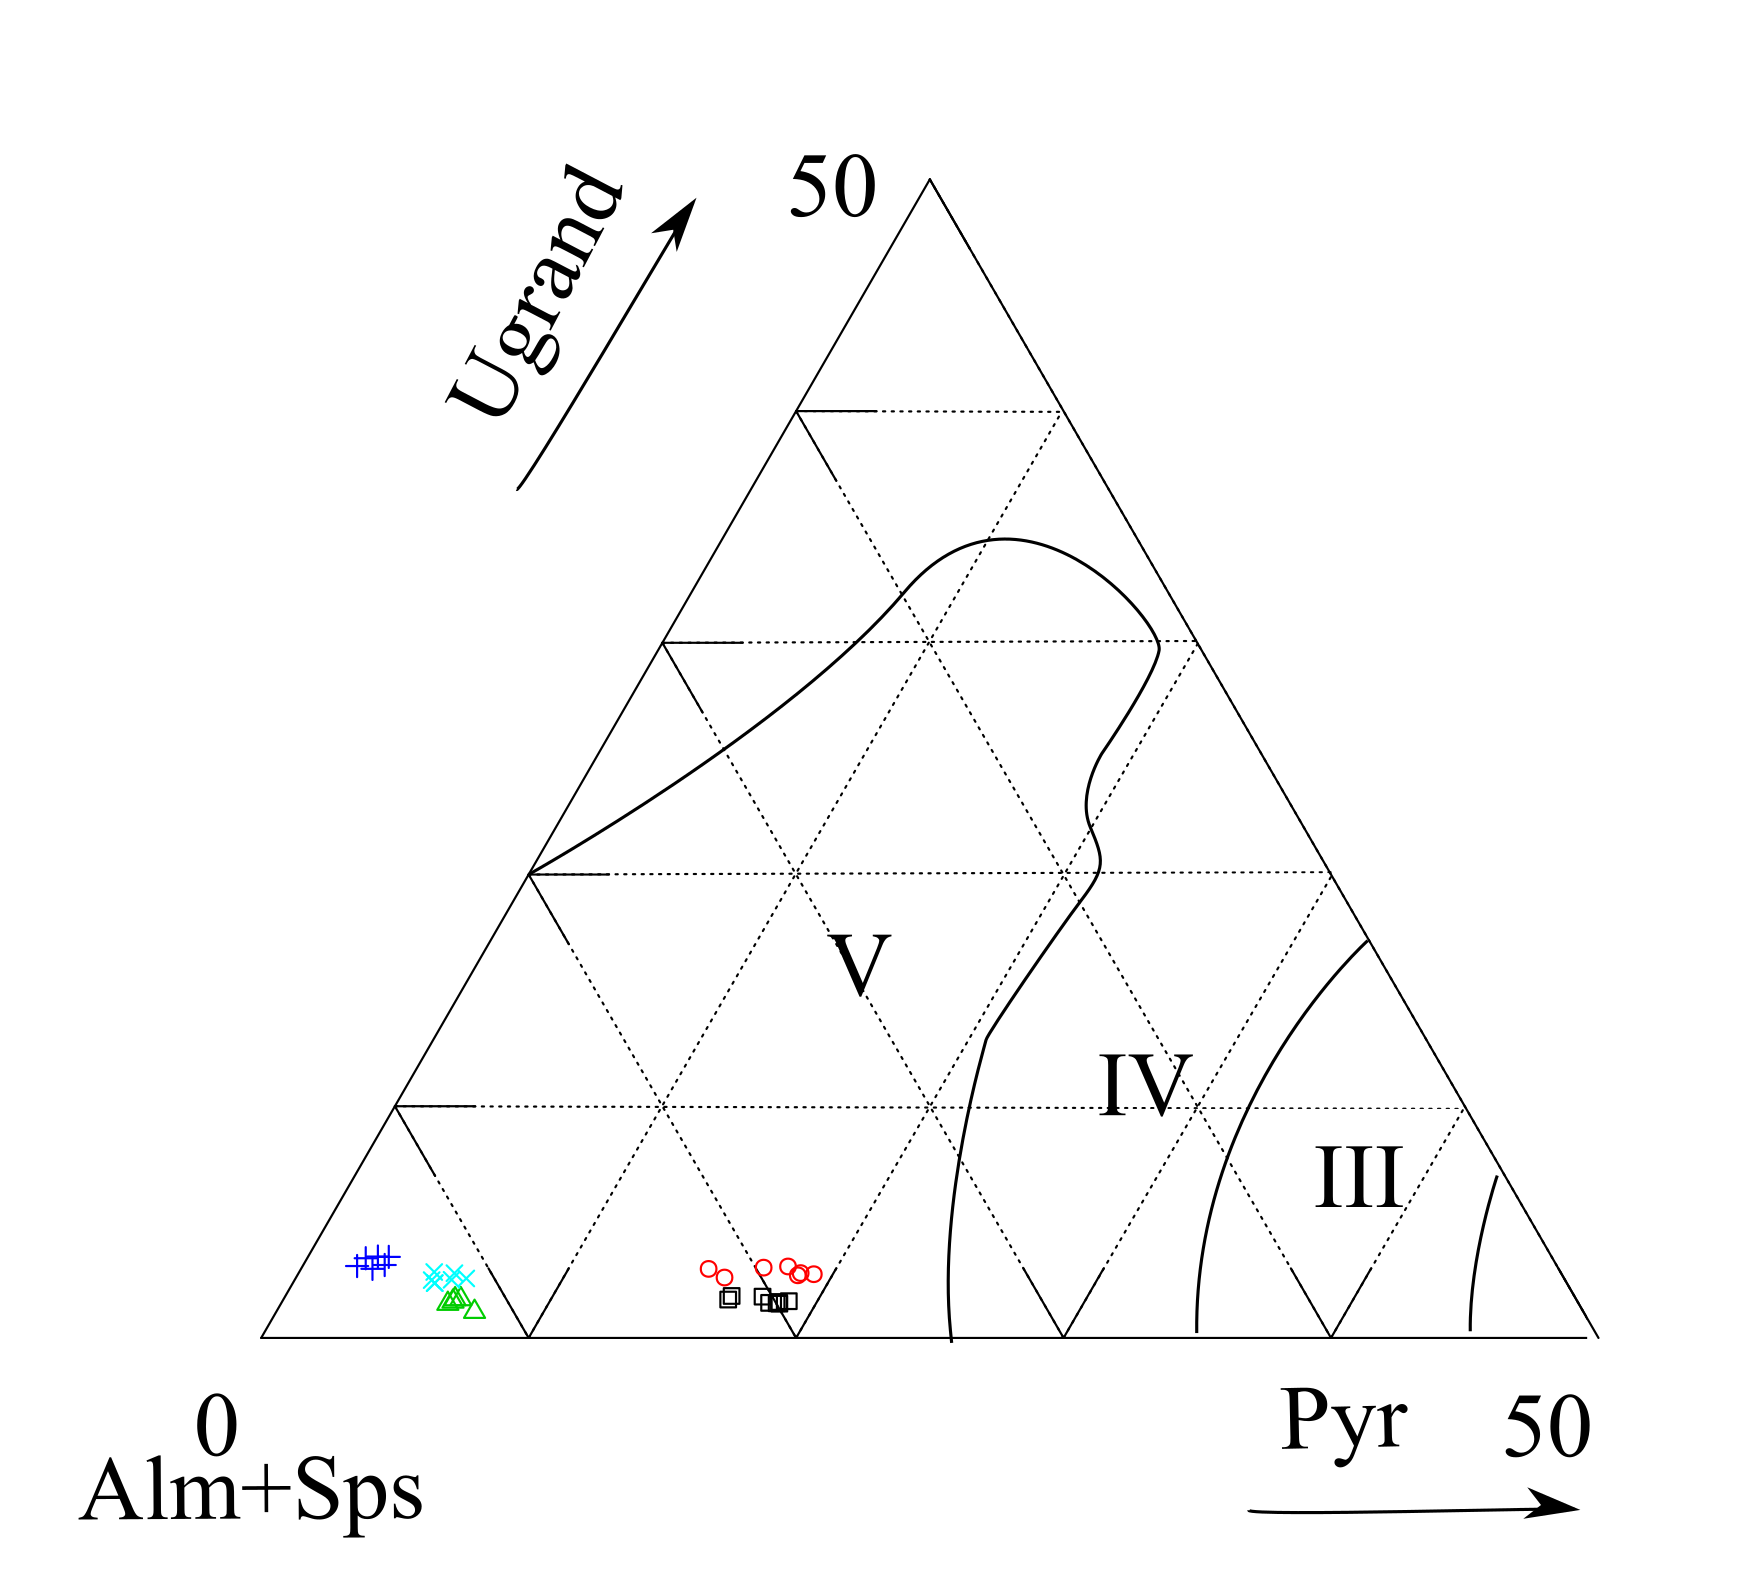
\includegraphics[width=1\textwidth]{authors/polzunenkov-fig3.png}
      \end{center}

        \caption{Состав гранатов на диаграмме А.\,И.~Сизых [3]. Поля составов граната: III~--- силлиманит-альмандин-ортоклазовой субфации,  IV~--- дистен-альмандин-мусковитовой  и  ставролит-дистен-альмандиновой субфации амфиболитовой фации, V~--- эпидот-амфиболитовой фации}
        \label{fig:polzunenkov-fig3}
    \end{minipage}


  \end{center}
\end{changemargin}

\end{figure}
